% THIS DOCUMENT IS TAILORED TO REQUIREMENTS FOR SCIENTIFIC COMPUTING.  IT SHOULDN'T
% BE USED FOR NON-SCIENTIFIC COMPUTING PROJECTS
\documentclass[12pt]{article}

\usepackage{amsmath, mathtools}
\usepackage{amsfonts}
\usepackage{amssymb}
\usepackage{graphicx}
\usepackage{colortbl}
\usepackage{xr}
\usepackage{hyperref}
\usepackage{longtable}
\usepackage{xfrac}
\usepackage{tabularx}
\usepackage{float}
\usepackage{siunitx}
\usepackage{booktabs}
\usepackage{caption}
\usepackage{pdflscape}
\usepackage{afterpage}
\usepackage{hyperref}
\usepackage[flushleft]{threeparttable}

\usepackage[round]{natbib}

%\usepackage{refcheck}

\hypersetup{
    bookmarks=true,         % show bookmarks bar?
      colorlinks=true,       % false: boxed links; true: colored links
    linkcolor=red,          % color of internal links (change box color with linkbordercolor)
    citecolor=green,        % color of links to bibliography
    filecolor=magenta,      % color of file links
    urlcolor=cyan           % color of external links
}

%% Comments

\usepackage{color}

\newif\ifcomments\commentstrue %displays comments
%\newif\ifcomments\commentsfalse %so that comments do not display

\ifcomments
\newcommand{\authornote}[3]{\textcolor{#1}{[#3 ---#2]}}
\newcommand{\todo}[1]{\textcolor{red}{[TODO: #1]}}
\else
\newcommand{\authornote}[3]{}
\newcommand{\todo}[1]{}
\fi

\newcommand{\wss}[1]{\authornote{blue}{SS}{#1}} 
\newcommand{\plt}[1]{\authornote{magenta}{TPLT}{#1}} %For explanation of the template
\newcommand{\an}[1]{\authornote{cyan}{Author}{#1}}

%% Common Parts

\newcommand{\progname}{ImgBeamer} % PUT YOUR PROGRAM NAME HERE
\newcommand{\authname}{Joachim de Fourestier} % AUTHOR NAMES                  

\usepackage{hyperref}
    \hypersetup{colorlinks=true, linkcolor=blue, citecolor=blue, filecolor=blue,
                urlcolor=blue, unicode=false}
    \urlstyle{same}
                                


% For easy change of table widths
\newcommand{\colZwidth}{1.0\textwidth}
\newcommand{\colAwidth}{0.13\textwidth}
\newcommand{\colBwidth}{0.82\textwidth}
\newcommand{\colCwidth}{0.1\textwidth}
\newcommand{\colDwidth}{0.05\textwidth}
\newcommand{\colEwidth}{0.8\textwidth}
\newcommand{\colFwidth}{0.17\textwidth}
\newcommand{\colGwidth}{0.5\textwidth}
\newcommand{\colHwidth}{0.28\textwidth}

% Used so that cross-references have a meaningful prefix
\newcounter{defnum} %Definition Number
\newcommand{\dthedefnum}{GD\thedefnum}
\newcommand{\dref}[1]{GD\ref{#1}}
\newcounter{datadefnum} %Datadefinition Number
\newcommand{\ddthedatadefnum}{DD\thedatadefnum}
\newcommand{\ddref}[1]{DD\ref{#1}}
\newcounter{theorynum} %Theory Number
\newcommand{\tthetheorynum}{T\thetheorynum}
\newcommand{\tref}[1]{TM\ref{#1}}
\newcounter{tablenum} %Table Number
\newcommand{\tbthetablenum}{T\thetablenum}
\newcommand{\tbref}[1]{TB\ref{#1}}
\newcounter{assumpnum} %Assumption Number
\newcommand{\atheassumpnum}{P\theassumpnum}
\newcommand{\aref}[1]{A\ref{#1}}
\newcounter{goalnum} %Goal Number
\newcommand{\gthegoalnum}{P\thegoalnum}
\newcommand{\gsref}[1]{GS\ref{#1}}
\newcounter{instnum} %Instance Number
\newcommand{\itheinstnum}{IM\theinstnum}
\newcommand{\iref}[1]{IM\ref{#1}}
\newcounter{reqnum} %Requirement Number
\newcommand{\rthereqnum}{P\thereqnum}
\newcommand{\rref}[1]{R\ref{#1}}
\newcounter{nfrnum} %NFR Number
\newcommand{\rthenfrnum}{NFR\thenfrnum}
\newcommand{\nfrref}[1]{NFR\ref{#1}}
\newcounter{lcnum} %Likely change number
\newcommand{\lthelcnum}{LC\thelcnum}
\newcommand{\lcref}[1]{LC\ref{#1}}
\newcounter{ucnum} %Likely change number
\newcommand{\ltheucnum}{UC\theucnum}
\newcommand{\ucref}[1]{UC\ref{#1}}

\usepackage{fullpage}

\newcommand{\deftheory}[9][Not Applicable]
{
\newpage
\noindent \rule{\textwidth}{0.5mm}

\paragraph{RefName: } \textbf{#2} \phantomsection 
\label{#2}

\paragraph{Label:} #3

\noindent \rule{\textwidth}{0.5mm}

\paragraph{Equation:}

#4

\paragraph{Description:}

#5

\paragraph{Notes:}

#6

\paragraph{Source:}

#7

\paragraph{Ref.\ By:}

#8

\paragraph{Preconditions for \hyperref[#2]{#2}:}
\label{#2_precond}

#9

\paragraph{Derivation for \hyperref[#2]{#2}:}
\label{#2_deriv}

#1

\noindent \rule{\textwidth}{0.5mm}

}

\begin{document}

\pagenumbering{gobble} % avoid page number on title page

\title{Software Requirements Specification for \progname: Scanning Electron Microscope Image Formation} 
\author{\authname}
\date{\today}
	
\maketitle

~\newpage

\pagenumbering{roman}

\tableofcontents

~\newpage

\section*{Revision History}

\begin{tabularx}{\textwidth}{p{3cm}p{2cm}X}
\toprule {\bf Date} & {\bf Version} & {\bf Notes}\\
\midrule
2023/02/03 & 1.0 & First version\\
2023/02/11 & 1.1 & Changes after review by domain expert\\
2023/02/15 & 1.2 & Changes after review by SRS secondary reviewer\\
2023/02/15 & 1.3 & Includes some changes after review by Dr. Smith\\
2023/02/17 & 1.3.1 & Added some missing definitions\\
2023/02/17 & 1.3.2 & Some changes needed for use with the VnV plan\\
\bottomrule
\end{tabularx}

~\newpage

\section{Reference Material}

This section records information for easy reference.

\subsection{Table of Units}

Throughout this document SI (Syst\`{e}me International d'Unit\'{e}s) is employed
as the unit system. In addition to the basic units, several derived units are
used as described below. For each unit, the symbol is given followed by a
description of the unit and the name.
~\newline

%\begin{table}[ht]
  \noindent \begin{tabular}{l l l} 
    \toprule		
    \textbf{symbol} & \textbf{unit} & \textbf{name}\\
    \midrule
    px & pixel & picture element \\
    \si{\nm} & length & nanometre (\num{d-9} m)\\
    \si{\um} & length & micrometre (\num{d-6} m)\\
    \bottomrule
  \end{tabular}
  %	\caption{SI Units}
%\end{table}

\subsection{Table of Symbols}

The table that follows summarizes the symbols used in this document along with
their units. The choice of symbols was made to be consistent with EM (Electron
Microscopy) literature and with existing documentation for EM systems. 
The symbols are listed in alphabetical order.

\renewcommand{\arraystretch}{1.2}
%\noindent \begin{tabularx}{1.0\textwidth}{l l X}
\noindent \begin{longtable*}{l l p{12cm}} \toprule
\textbf{symbol} & \textbf{unit} & \textbf{description}\\
\midrule 
$d_p$ & \si[per-mode=symbol] {\nm} & probe diameter (size)\\
$d_i$ & \si[per-mode=symbol] {\nm} & probe step size in image space\\
$d_o$ & \si[per-mode=symbol] {\nm} & probe step size in object space\\
$\eta$ & dimensionless & BSE yield \\
$\delta$ & dimensionless & SE yield \\
$I_{n\times m}$ & 8-bit gray level & Image intensity matrix that has $n$ rows and $m$ columns.\\
$M_{n\times m}$ & Boolean & Mask / stencil matrix that has $n$ rows and $m$ columns.\\
$R_{n\times m}$ & 8-bit gray level & Resulting image intensity matrix that has $n$ rows and $m$ columns.\\
\bottomrule
\end{longtable*}

\subsection{Abbreviations and Acronyms}

\renewcommand{\arraystretch}{1.2}
\begin{tabular}{l l} 
  \toprule		
  \textbf{symbol} & \textbf{description}\\
  \midrule 
  2D & two-dimensional\\
  3D & three-dimensional\\
  A & Assumption\\
  BSE & Backscattered Electron\\
  CCD & Charge Coupled Device\\
  DD & Data Definition\\
  EM & Electron Microscopy\\
  FOV & Field of View\\
  GD & General Definition\\
  GS & Goal Statement\\
  IM & Instance Model\\
  LC & Likely Change\\
  LM & Light Microscopy\\
  PS & Physical System Description\\
  R & Requirement\\
  ROI & Region of Interest\\
  SE & Secondary Electron\\
  SEM & Scanning Electron Microscope\\
  SRS & Software Requirements Specification\\
  TM & Theoretical Model\\
  \progname{} & SEM image formation demo tool\\
  \bottomrule
\end{tabular}\\

\newpage

\pagenumbering{arabic}

\section{Introduction}

Images formed by SEM (Scanning Electron Microscope) are created using a 
specific process where the image quality can be greatly influenced by the 
imaging parameters (e.g., spot profile, pixel size). Since the quality of 
an image is very often evaluated subjectively by an experienced microscope 
user, the motivation of this software project ``\progname{}'' is to provide a way to visualize 
qualitatively the said influence without the need of a physical instrument.
Incorrectly adjusting the imaging parameters could lead to a loss of information 
or misinterpretation. The issue is further explained in the 
Problem Statement document. Some figures expanding on the subject can be
found in section \ref{sec_phySystDescrip}.
An underlying goal is also to prove or disprove if 
there is a ``rule of thumb'' for the optimal spot-to-pixel size ratio.

\subsection{Purpose of Document}

This document serves as the software requirements specification. The details of the 
requirements, limitations, definitions, models to be used are laid out explicitly 
within this document.

\subsection{Scope of Requirements} 

The scope of the requirements is restricted to only the image 
formation process used in SEMs, more specifically the image processing from 
signal to an image or visual representations. It does not cover election-sample 
interactions or CCD (charge-coupled device) detector voltage to signal value 
conversion. See the assumptions section (Section~\ref{sec_assumpt}) for further 
details.

\subsection{Characteristics of Intended Reader} \label{sec_IntendedReader}

The intended reader of this document should have a basic understanding of 
electron-optics concepts used by an SEM. This can be equated to standard level 
two university physics (optics, electricity, magnetism, thermodynamics and 
modern physics) along with a standard undergraduate course related to materials 
characterization (concepts such as backscattered electrons, mean free path, and 
electron density). The reader should have a basic understanding of two-dimensional 
image processing techniques and level one university linear algebra (matrices).

\subsection{Organization of Document}

This document contains an introduction to the software and its goals. It is 
meant to be a reference document to the readers and is based on an SRS template from \citet{SmithAndLai2005, SmithEtAl2007}. The document includes a 
description of the scope, a detailed list of the terminology, definitions, and 
models used, as well as a more specific and detailed description of the problem 
and its solutions. This document also defines the requirements, as well as the  
likely changes and traceability details.

\section{General System Description}

This section provides general information about the system. It identifies the
interfaces between the system and its environment, describes the user
characteristics and lists the system constraints.

\subsection{System Context}

The general input and output pattern of the \progname{} software is shown in the 
system context diagram (figure \ref{Fig_SystemContext}). This section also 
includes the responsibilities of the user and the software.

\setlength{\belowcaptionskip}{-30pt}
\begin{figure}[h!]
\begin{center}
 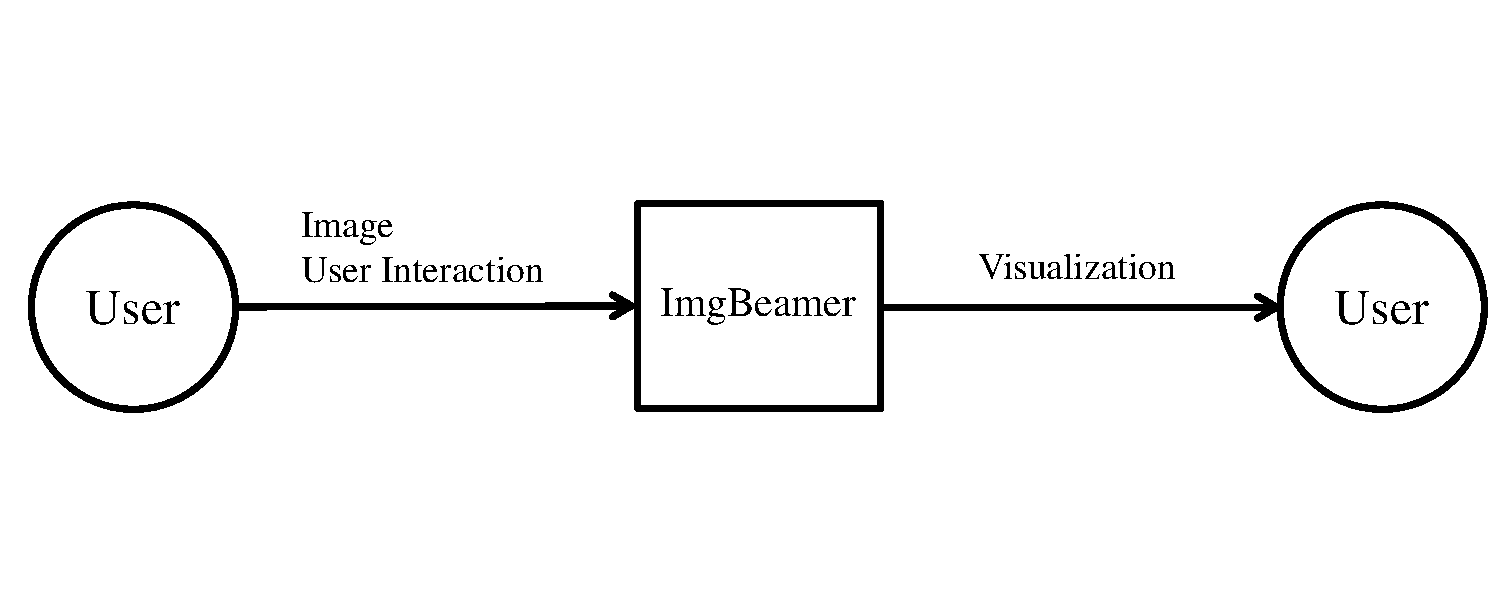
\includegraphics[width=0.8\textwidth]{SystemContextFigure}
\caption{System Context}
\label{Fig_SystemContext} 
\end{center}
\end{figure}
\setlength{\belowcaptionskip}{10pt}

\begin{itemize}

  \item User Responsibilities:
  \begin{itemize}
    \item Provide an image of sufficient size (see \ref{sec_DataConstraints}), such that there is enough detail.
    \item Provided a ground truth image that should be free of distortions (e.g., from FOV edges, depth of field, ``charging'', insufficient focus, astigmatism, etc.).
    \item Be able to interact with the software's graphical user interface using a computer mouse, keyboard and monitor.
    \item Provide realistic spot profiles (size and shape).
    \item Run the software on a platform or system with sufficient resources to process computer graphics.
  \end{itemize}

  \item \progname{} Responsibilities:
  \begin{itemize}
    \item Provide the ability load or change the input ground truth image.
    \item Detect and warn about invalid or corrupt image files.
    \item Set reasonable limits (minimum and maximum dimensions) on the spot profile. 
    \item Be responsive, taking user input at anytime and prevent locking or freezing of the graphical user interface as much as possible.
    \item Have reasonable starting default inputs and values.
    \item Display the image quality metric.
    \item Provide the ability to export the resulting images.
  \end{itemize}

\end{itemize}

\subsection{User Characteristics} \label{SecUserCharacteristics}

The \progname{} software end user is anyone that has used an SEM or is learning about them. 
This ranges from a university undergraduate science student whose curriculum includes 
EM (Electron Microscopy), to experienced SEM operators or even to experts in the field of EM. 
The software end users also include those described in Section~\ref{sec_IntendedReader} 
(intended readers of this document). That said, neither image processing nor linear algebra knowledge 
is required to use the software. 

\subsection{System Constraints}

The real world design constraints are to be listed here, but there are none.

\section{Specific System Description}

This section first presents the problem description, which gives a high-level
view of the problem to be solved. This is followed by the solution characteristics
specification, which presents the assumptions, theories, definitions and finally
the instance models.

\subsection{Problem Description} \label{Sec_pd}

\progname{} is intended to help visualize and understand the influence of the 
spot profile and pixel size. It should be able to help determine the optimal 
spot-to-pixel-size ratio (see fig.~\ref{fig_samp_ratios} and \ref{fig_samp_scenarios}).

\subsubsection{Terminology and Definitions}

This subsection provides a list of terms that are used in the subsequent
sections and their meaning, with the purpose of reducing ambiguity and making it
easier to correctly understand the requirements:

\begin{center}
    \noindent
    \begin{longtable}{p{4.25cm} p{11.25cm}} 
        \toprule
        \textbf{Terminology} & \textbf{Definition}\\
        \midrule
        Backscattered Electron & An electron that is elastically scattered backwards to the initial direction of travel as a result of electron-sample interactions between the beam and the sample. \\
        
        Beam & The continuous focused stream of electrons accelerated at high speeds down the column of an electron microscope. \\

        Bit Depth & It is the range of the value (intensity or color) of a pixel. Specifically, it is the maximum number of bits used to represent said value. \\
        
        Brightness & The intensity value (or perceived luminance for colours) of a signal, point (or pixel), or area within an image. \\
        
        Contrast & The difference or distinguishable quality of an intensity (or colour) or brightness value of a point (or pixel) from another point in an image.\\
        
        Electron-Sample\newline Interactions & The interactions as a result of electrons from the beam hitting the sample surface leading to an electron collision cascade. This in produces various emissions such as x-rays, BSEs, and SEs. \\
        
        Electron Microscopy & The practice of microscopes that specifically use electrons as the source of illumination to produce an image or signal.  \\
        
        Exact-sampling & The sampling size or rate that matches the specificity of the targeted resolution. In the context of this document, this is when the size of the probe that matches the size of the pixel. \\
        
        Field of View & The observable or visible extent given by the microscope and varies with magnification. \\
        
        Ground Truth & The data or information that is considered as the source or reference standard of truth. \\
        
        Image & A representation of visual information that can be represented by 2D matrix where each cell represents a pixel with a specific value (representative of intensity or colour). -- \\
        
        Image Quality & The perceived clarity, amount of information or detail representative of reality that is contained within an image. \\
        
        Image Resolution & The size dimensions (width and height) of an image. Typically, it is defined in pixels. \\
        
        Interaction Volume & The volume within the sample in which there are electron-sample interactions caused by the beam coming into contact with the surface of the sample. \\
        
        Light Microscopy & The practice of microscopes that specifically use light as the source of illumination to produce an image or signal. \\

        Mean Free Path & The average distance within a system that a particle can travel before it collides with other particles.\\
        
        Nyquist Limit & More formally known as the ``Nyquist-Shannon'' sampling limit is the minimum sampling rate at which all the essential information is captured when discretizing a continuous signal, resulting in little to no distortions. \\
        
        Over-sampling & This is a sampling rate or size that is too large where the specificity or origin of the information is lost. This generally results in increased confidence, but at a loss of precision.\\
        
        Pixel Size & The size or dimensions of one cell within a raster grid. \\
        
        Probe & Generally interchangeable with ``beam''. Contextually within this document, it is the final part of the beam that comes into contact with the surface of the sample (being analyzed within the microscope) forming a ``spot'' with a targeted size and shape. \\
        
        Raster Grid & A scanning pattern with a defined and repeated cell size. \\
        
        Region of Interest & A defined 2D area in both position, size, and shape on a sample. \\
        
        Resolution & As defined by the Rayleigh criterion, it is the minimum distance by which two points or features can be distinguished. \\
        
        Secondary Electron & An electron that emitted from the sample as a result of inelastic electron-sample interactions between the beam and the sample. These can be weakly bounded valence electrons or conduction band electrons. \\
        
        Signal-to-Noise Ratio & The amount of information (signal) considered useful or representative of reality versus the amount of noise. \\

        Spot Content & The area covered and sampled by the probe to produce a signal value. \\

        Spot Layout & The regular arrangement, sizing, and positioning of the spots and the raster grid used for imaging the sample surface. (ex. see fig. \ref{fig_sampling}) \\
        
        Spot Shape & The overall shape of the spot or probe, whether is it a perfect circle or elongated ellipse, or even a halo or ring. \\
        
        Spot Size & The overall diameter or average feret/caliper diameter of the probe. \\
        
        Step Size & The length or distance of a ``pixel'' by which the probe is moved or deflected when raster scanning the surface of a sample. \\
        
        Subregion & A region or area usually contained within the current FOV. This can also be synonymous to ROI. \\

        Under-sampling & This is a sampling rate or size that is too small where the specificity or origin of the information is more restricted. This generally results in increased precision, but at a loss of confidence, or even accuracy. \\
        \bottomrule
    \end{longtable} 
\end{center}


\subsubsection{Physical System Description} \label{sec_phySystDescrip}

The basic principle of the SEM image formation process is to scan an electron beam over the surface 
of the sample (fig.~\ref{fig_ebeam}) at discrete locations: cells of a raster or scan grid. A signal (e.g., BSEs, SEs) is 
produced as the beam dwells over each cell (representing a pixel in the resulting image). This 
signal is then collected by detectors to calculate a value (or intensity) to fill the corresponding
pixel in the resulting image. The area sampled (spot content) depends on the spot's (produced by the beam) size and 
shape (see fig.~\ref{fig_sampling}). \\

The physical system of \progname{}, as shown in Figure \ref{fig_ebeam} and \ref{fig_sampling},
includes the following elements:

\begin{itemize}

\item[PS1:] The sample that is being imaged or studied.

\item[PS2:] An SEM that includes a BSE and/or SE detector. The electron beam interacts with the sample surface in high-vacuum producing various signals.

\end{itemize}

\setlength{\belowcaptionskip}{-30pt}
\begin{figure}[h!]
\begin{center}
{
 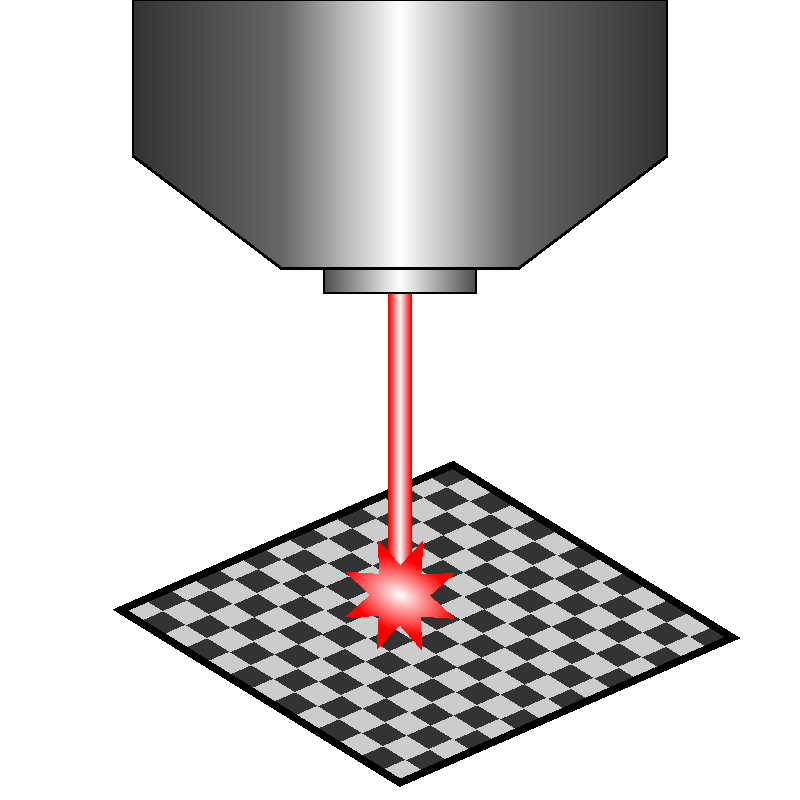
\includegraphics[width=0.27\textwidth]{figures/e_beam.pdf}
}
\caption{\label{fig_ebeam} Schematic drawing of an electron beam hitting the sample surface within an SEM chamber. (Image from: \url{https://github.com/joedf/ImgBeamer})}
\end{center}
\end{figure}
\setlength{\belowcaptionskip}{10pt}

\begin{figure}[h!]
\begin{center}
{
 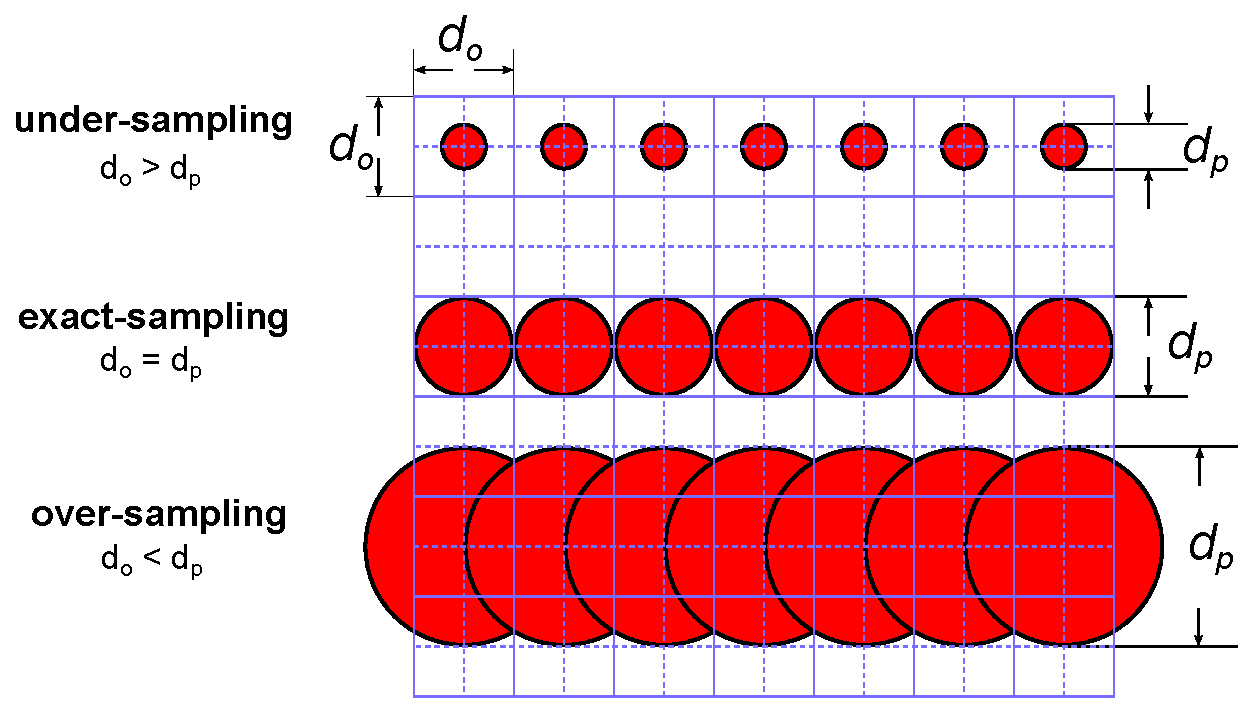
\includegraphics[width=0.77\textwidth]{figures/sampling.pdf}
}
\caption{\label{fig_sampling} Schematic of the three sampling scenarios (under-sampling, exact-sampling, and over-sampling) and a visual representation of the pixel grid, $d_p$, and $d_o$. The dashed lines are to help visualize the center of each pixel cell. Adapted from \citet{lifshin_improving_2014}}
\end{center}
\end{figure}

\begin{landscape}
\setlength{\belowcaptionskip}{-30pt}
\vspace*{\fill}
\begin{figure}[h!]
\begin{center}
{
 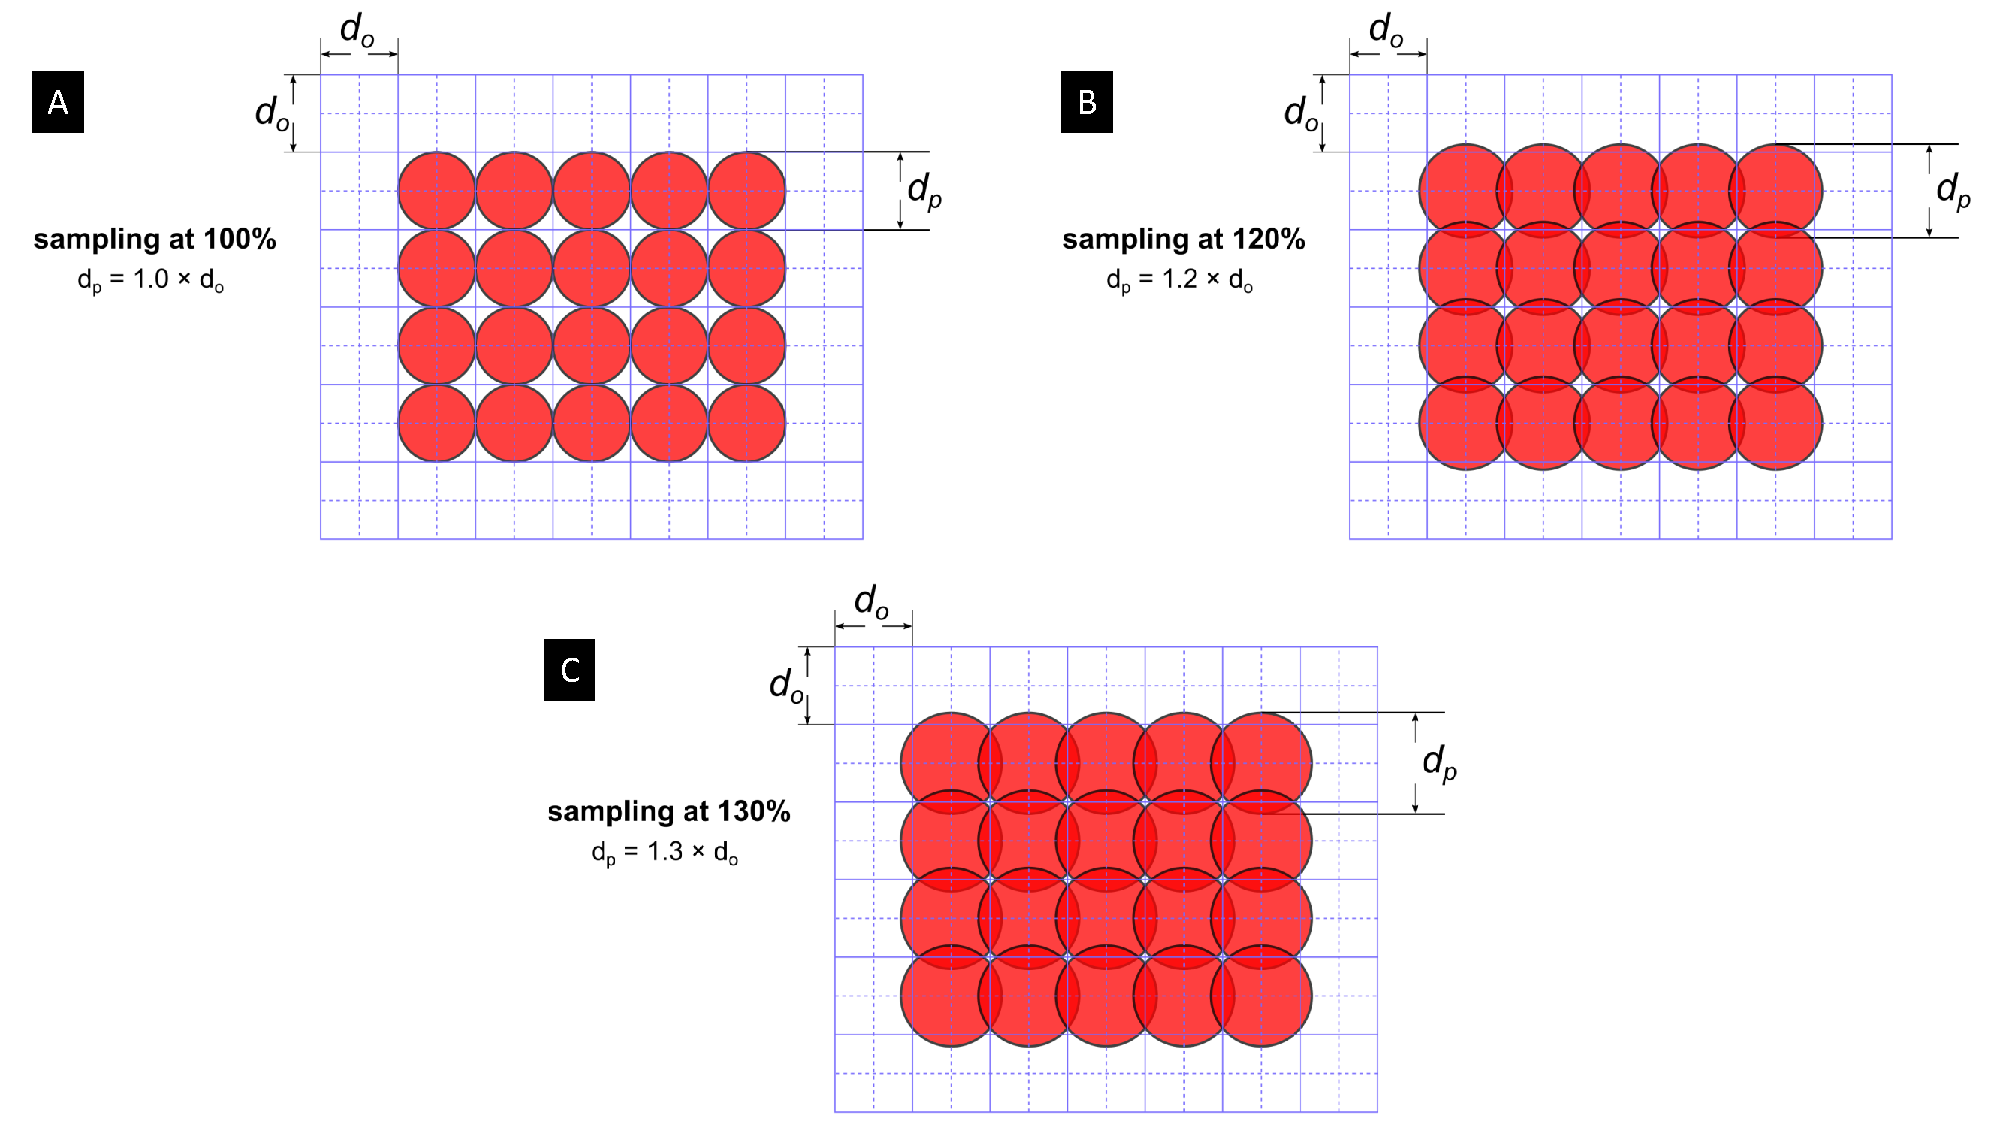
\includegraphics[width=1.3\textwidth]{figures/spot_ratio/sampling_ratios.pdf}
}
\caption{\label{fig_samp_ratios} Different scenarios of the spot sizes (represented by the red circles) are presented to show the area coverage and overlap that would occur in a raster scan. [A] represents exact-sampling (as explained in figure \ref{fig_sampling}), where there are considerable gaps between the spot locations. In [B], the gaps are small meaning little loss in area coverage, but there is some overlap. In [C], as we approach to a spot diameter that is equal to the square diagonal ($\sqrt{2} \approx 1.4142$), the gaps are significantly reduced as the overlap grows to a geometric maximum.}
\end{center}
\end{figure}
\vspace*{\fill}
\setlength{\belowcaptionskip}{10pt}
\end{landscape}

Depending on how large the spot size is, the surface area coverage (or spot content) will vary. As shown in
figure \ref{fig_samp_ratios}, a circular spot cannot cover the entire area without overlap. However,
when the spot size is small, there is no overlap, but there are significant gaps where potentially 
means a loss of in formation. There is a balance between the overlaps and the gaps. 
In figure \ref{fig_samp_scenarios}, we can see how this balance can affect the reconstructed image's
sharpness versus its amount of detail or visual information.

~\newline

\begin{figure}[h!]
\begin{center}
{
 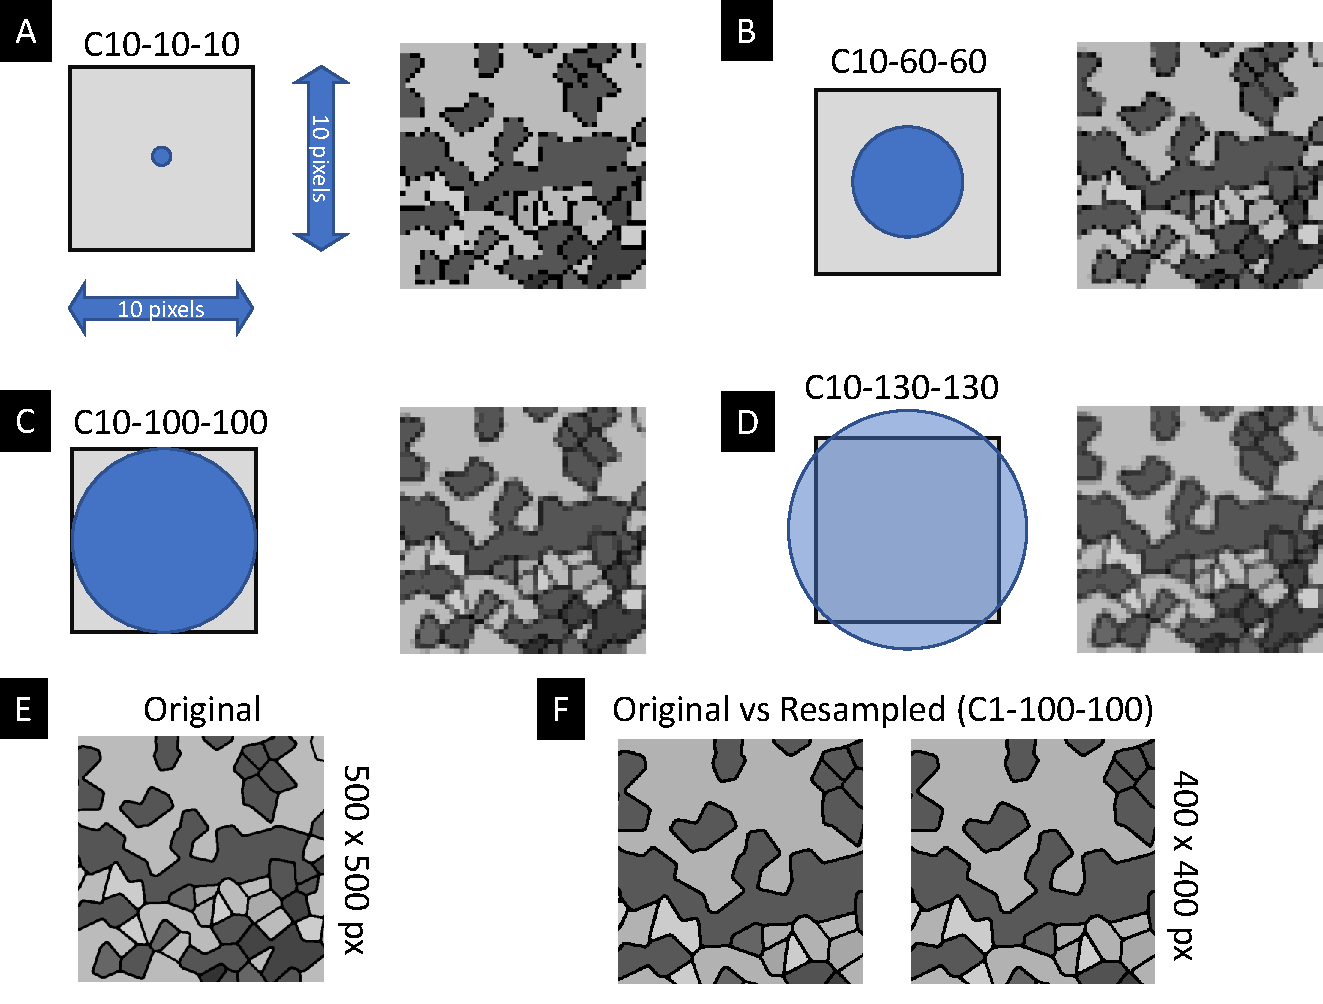
\includegraphics[width=0.8\textwidth]{figures/spot_ratio/sampling_scenarios.pdf}
}
\caption{\label{fig_samp_scenarios} Different sampling scenarios are presented here (A-D). The blue circles represent the imaging or beam spot. The notation C10 represents a square cell size of 10 by 10 pixels. The following numbers are percentages of the spot diameter size with respect to the cell width. For example in [D], we have a spot where its diameter is 130\% of the cell's width. [E] represents the original image that was resampled. It is a virtual BSE image representing a crystalline sample. [F] shows a ``high-fidelity'' reconstructed image meaning the pixel size is one-to-one with exact-sampling (100\%). There is no perceivable difference.}
\end{center}
\end{figure}

\newpage

In more extreme cases as shown in figure \ref{fig_samp_scenarios_extra} (exaggerated for clarity), 
if there is over-sampling in one direction and under-sampling in another can create the effect of 
astigmatism. Whereas in the scenario where we grossly over-sample in all directions, we obtain the 
effect of an unfocused image.

~\newline

\begin{figure}[h!]
\begin{center}
{
 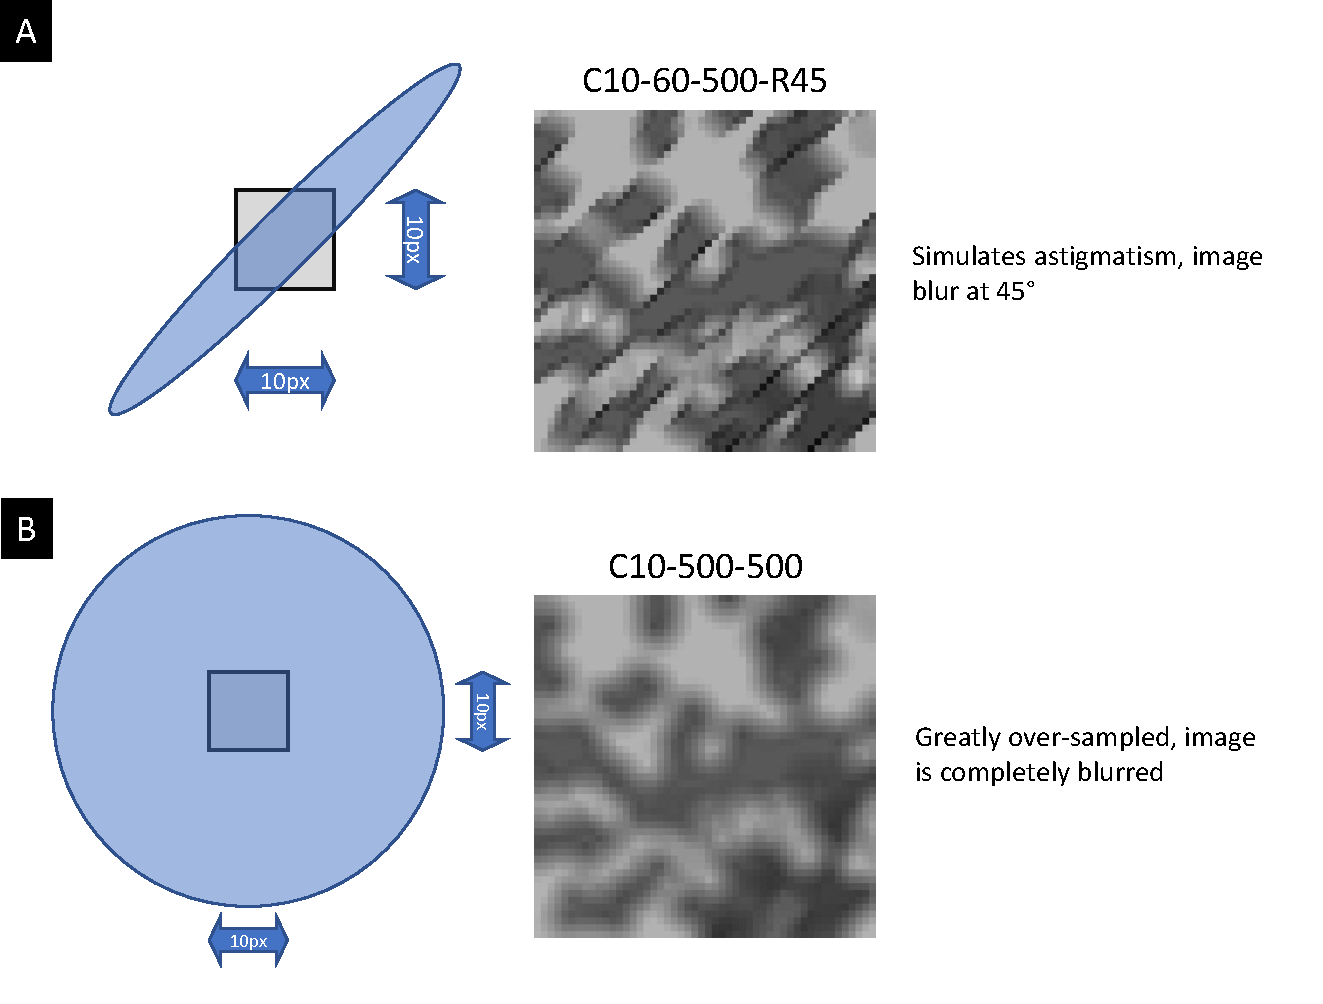
\includegraphics[width=0.8\textwidth]{figures/spot_ratio/sampling_scenarios-extra.pdf}
}
\caption{\label{fig_samp_scenarios_extra} Following the same notation as explained in figure \ref{fig_samp_scenarios}, here are two extra examples (A and B). [A] represents the scenario of astigmatism that is dominant at a 45-degree angle. [B] represents the scenario of defocus (or insufficient focus).}
\end{center}
\end{figure}

\newpage
\clearpage

\subsubsection{Goal Statements}

\noindent Given an image (ground truth) and imaging parameters (e.g., spot size, spot shape, pixel size), the goal statements are:

\begin{itemize}

\item[GS\refstepcounter{goalnum}\thegoalnum \label{G_reprocess}:] {
Reprocess the image following the SEM image formation process.
}

\item[GS\refstepcounter{goalnum}\thegoalnum \label{G_metric}:] {
Provide a quantitative metric of relative image quality of the resulting image.
}

\item[GS\refstepcounter{goalnum}\thegoalnum \label{G_visualize}:] {
Visualize the effects of changing the imaging parameters.
}

\item[GS\refstepcounter{goalnum}\thegoalnum \label{G_export}:] {
Export the reprocessed images.
}

\end{itemize}

\subsection{Solution Characteristics Specification}

This section provides the assumptions, instance models, theoretical models, general definitions, and data constraints. The information specified in this section is intended to reduce ambiguities and reduce the problem into clear logical or mathematical terms. \\

The instance models that govern \progname{} are presented in
Subsection~\ref{sec_instance}. The information to understand the meaning of the
instance models and their derivation is also presented, so that the instance
models can be verified.

\subsubsection{Assumptions} \label{sec_assumpt}

This section simplifies the original problem and helps in developing the
theoretical model by filling in the missing information for the physical
system. The numbers given in the square brackets refer to the theoretical model
[TM], general definition [GD], data definition [DD], instance model [IM], or
likely change [LC], in which the respective assumption is used.

\begin{itemize}

\item[A\refstepcounter{assumpnum}\theassumpnum \label{A_sampleSolid}:] The sample 
surface is solid.

\item[A\refstepcounter{assumpnum}\theassumpnum \label{A_sampleZ}:] The sample 
material is made of atoms with atomic numbers greater than 3 (lithium and lighter elements are not detectable in SEM).

\item[A\refstepcounter{assumpnum}\theassumpnum \label{A_beam}:] The electron 
beam is ideal (meaning stable and collimated meaning all the electrons are 
traveling parallel to each other down towards the sample surface within high 
vacuum for optimal mean free path).

\item[A\refstepcounter{assumpnum}\theassumpnum \label{A_inputImage}:] The input 
image of the sample is considered to have infinite resolution representative of reality: ground truth.

\item[A\refstepcounter{assumpnum}\theassumpnum \label{A_yield}:] The signal yields (such as BSEs and SEs, see \ddref{DD_yield})
are high enough to produce an image meaning optimal SNR (enough signal, 
contrast [\tref{T_contrast}] and noise is low).

\item[A\refstepcounter{assumpnum}\theassumpnum \label{A_reality}:] The image 
produced by the SEM (see \ddref{DD_signalImage}) as the electron raster scan the sample surface is an 
approximate representation of reality.

\item[A\refstepcounter{assumpnum}\theassumpnum \label{A_deflectionLimit}:] The beam's deflection 
space (\tref{T_deflectionSpace}) will not be a limiting factor in how wide the coverage area 
of the sample surface.

\end{itemize}

\subsubsection{Theoretical Models}\label{sec_theoretical}

This section focuses on the general equations and laws that \progname{} is based
on.
~\newline

\noindent
\begin{minipage}{\textwidth}
\renewcommand*{\arraystretch}{1.5}
\begin{tabular}{| p{\colAwidth} | p{\colBwidth}|}
  \hline
  \rowcolor[gray]{0.9}
  Number& TM\refstepcounter{theorynum}\thetheorynum \label{T_meanfreepath}\\
  \hline
  Label& \bf Mean Free Path\\
  \hline
  Equation &
    $\lambda = \frac{RT}{\sqrt{2}\pi d^{2}N_AP}$ \\[3pt]
  \hline
  Description
    & $\lambda$ is the mean free path (\si{m}) \\
    & $R$ is the universal gas constant = $8.3145$ \si{J/mol.K} \\
    & $T$ is the temperature (\si{K}) \\
    & $d$ is the molecular diameter (\si{m}) \\
    & $P$ is the pressure (\si{Pa}) \\
    & $N_A$ is Avogadro's number = $6.0221 \times 10^{23}$ \si{\per\mol} \\
  \hline
  Notes & See \aref{A_beam}. \\
  \hline
  Sources& \url{http://hyperphysics.phy-astr.gsu.edu/hbase/Kinetic/menfre.html} \\
  \hline
  Ref.\ By & -- \\
  \hline
\end{tabular}
\end{minipage}\\
~\newline

\noindent
\begin{minipage}{\textwidth}
\renewcommand*{\arraystretch}{1.5}
\begin{tabular}{| p{\colAwidth} | p{\colBwidth}|}
  \hline
  \rowcolor[gray]{0.9}
  Number& TM\refstepcounter{theorynum}\thetheorynum \label{T_contrast}\\
  \hline
  Label& \bf Contrast\\
  \hline
  Equation & $C_{tr} = (S_{2} - S_{1}) / S_{2}$ \\
  \hline
  Description
    & $C_{tr}$ This is proportion or level of contrast or difference in signal. It is dimensionless. \\
    & $S$ is the emitted signal strength or intensity (see \ddref{DD_yield}). \\
    & $S_{1}$ is one signal at one location (e.g., pixel). \\
    & $S_{2}$ is another signal at a different location to be compared with $S_{1}$ 
    and should the larger value of the two signals. \\
  \hline
  Notes
    & $S_{2} > S_{1}$ \\
  \hline
  Sources& \cite{goldstein_textbook_2018}, \cite{lifshin_improving_2014} \\
  \hline
  Ref.\ By & \aref{A_yield} \\
  \hline
\end{tabular}
\end{minipage}\\
~\newline

\noindent
\begin{minipage}{\textwidth}
\renewcommand*{\arraystretch}{1.5}
\begin{tabular}{| p{\colAwidth} | p{\colBwidth}|}
  \hline
  \rowcolor[gray]{0.9}
  Number& TM\refstepcounter{theorynum}\thetheorynum \label{T_mag}\\
  \hline
  Label& \bf Magnification\\
  \hline
  Equation & $M = \frac{d_i}{d_o}$ \\
  \hline
  Description
    & $M$ is the magnification ratio (unitless) \\
    & $d_i$ is the probe step size in image space \\
    & $d_o$ is the probe step size in object space \\
  \hline
  Notes & The input (ground truth) should be large enough and sufficient detail, see \aref{A_inputImage}. \\
  \hline
  Sources& \cite{lifshin_improving_2014} \\
  \hline
  Ref.\ By & -- \\
  \hline
\end{tabular}
\end{minipage}\\
~\newline

\noindent
\begin{minipage}{\textwidth}
\renewcommand*{\arraystretch}{1.5}
\begin{tabular}{| p{\colAwidth} | p{\colBwidth}|}
  \hline
  \rowcolor[gray]{0.9}
  Number& TM\refstepcounter{theorynum}\thetheorynum \label{T_deflectionSpace}\\
  \hline
  Label &\bf Deflection Space (or area / field)\\
  \hline
  Description
    & The deflection space is the area bounds in which the beam can be redirected 
    or oriented using deflection coils. It can be expressed in real world units, 
    but this can vary between SEMs. \\
    & From an imaging perspective, it can be generalized as a normalized unit 
    square coordinate system where the top left is (-0.5, -0.5), the center is 
    (0.0, 0.0), and the bottom right is (0.5, 0.5).
    \\
  \hline
  Source & \cite{goldstein_image_2018} \\
  \hline
  Ref.\ By & \aref{A_deflectionLimit}, \dref{GD_grid} \\
  \hline
\end{tabular}
\end{minipage}\\

\newpage

\subsubsection{General Definitions}\label{sec_gendef}

This section collects the laws and equations that will be used in building the
instance models.

~\newline

\noindent
\begin{minipage}{\textwidth}
\renewcommand*{\arraystretch}{1.5}
\begin{tabular}{| p{\colAwidth} | p{\colBwidth}|}
  \hline
  \rowcolor[gray]{0.9}
  Number& GD\refstepcounter{defnum}\thedefnum \label{GD_grid}\\
  \hline
  Label &\bf Raster or Scan Grid\\
  \hline
  Units & px (pixels) \\
  \hline
  Equation & $G(x,y): \{ x \ge 0, y \ge 0 \}$ \\
  \hline
  Description
    & $G$ is the grid pattern applied to the sample surface within the FOV and 
    spanning within deflection space (\tref{T_deflectionSpace}) of the SEM. \\
    & Each cell is a discrete $(x,y)$ location over which the beam scans over to 
    produce a signal. These signals are then collected by detectors to generate 
    an image. \\
    & Each cell represents a picture element or ``pixel''. \\
    & By convention, pixels are square, but this is not a necessity. That said, 
    non-square pixels may lead to unfaithful or distorted representations, see 
    \aref{A_reality} and \cite{goldstein_image_2018}. \\
    & The size of a pixel can be expressed in \si{\nm}, \si{\um}, or even a 
    percentage of the FOV. \\
  \hline
  Source & \cite{goldstein_image_2018} \\
  \hline
  Ref.\ By & -- \\
  \hline
\end{tabular}
\end{minipage}\\
~\newline

\newpage

\subsubsection{Data Definitions}\label{sec_datadef}

This section collects and defines all the data needed to build the instance
models. The dimension of each quantity is also given.

~\newline

\noindent
\begin{minipage}{\textwidth}
\renewcommand*{\arraystretch}{1.5}
\begin{tabular}{| p{\colAwidth} | p{\colBwidth}|}
  \hline
  \rowcolor[gray]{0.9}
  Number& DD\refstepcounter{datadefnum}\thedatadefnum \label{DD_yield}\\
  \hline
  Label& \bf Signal yield / intensity \\
  \hline
  Symbol & $\eta$ (for BSE), $\delta$ (for SE), $Y$ (for general) \\
  \hline
  Units & dimensionless \\
  \hline
  Equation & $Y_{signal} = N_{signal} / N_{B}$ \\
  \hline
  Description
    & $Y_{signal}$ is the intensity relative to the incident beam. \\
    & $N_{signal}$ is the number of scattered or emitted electrons. \\
    & $N_{B}$ is the number of (primary) incident electrons from the beam. \\
  \hline
  Notes
    & The $signal$ can BSE or SE. \\
    & There assumptions related to the beam, the signal produced, and sample nature, 
    see \aref{A_sampleZ}, \aref{A_beam}, and \aref{A_yield}. \\
  \hline
  Sources& \cite{goldstein_textbook_2018} \\
  \hline
  Ref.\ By & \ddref{DD_signalImage}, \tref{T_contrast}, \aref{A_yield} \\
  \hline
\end{tabular}
\end{minipage}\\
~\newline

\noindent
\begin{minipage}{\textwidth}
\renewcommand*{\arraystretch}{1.5}
\begin{tabular}{| p{\colAwidth} | p{\colBwidth}|}
  \hline
  \rowcolor[gray]{0.9}
  Number& DD\refstepcounter{datadefnum}\thedatadefnum \label{DD_signalImage}\\
  \hline
  Label& \bf Signal Image \\
  \hline
  Symbol & $I_{n\times m}$ \\
  \hline
  Units & intensity / ratio - unitless \\
  \hline
  Description
    & Each cell represents a pixel with a signal intensity (see \ddref{DD_yield}) or brightness value 
    where the range depends on the bit depth. \\
    & A bit depth of 8 is 0 to 255 (0xFF), and 16 is 0 to 65535 (0xFFFF). \\
    & We assume (see \aref{A_yield}) there's enough signal that can be detected, 
    as a $0$ represents no or ``undetected'' signal.\\
  \hline
  Sources& \cite{goldstein_textbook_2018} \\
  \hline
  Ref.\ By & \iref{IM_bitblt}, \aref{A_reality} \\
  \hline
\end{tabular}
\end{minipage}\\
~\newline

\newpage

\subsubsection{Instance Models} \label{sec_instance}    

This section transforms the problem defined in Section~\ref{Sec_pd} into 
one which is expressed in mathematical terms. It uses concrete symbols defined 
in Section~\ref{sec_datadef} to replace the abstract symbols in the models 
identified in Sections~\ref{sec_theoretical} and~\ref{sec_gendef}.

The goal of reprocessing an image \gsref{G_reprocess} will be solved by \iref{IM_bitblt}. The goal of providing an image quality metric will be solved by \iref{IM_imageMetric}.  

~\newline

%Instance Model 1

\noindent
\begin{minipage}{\textwidth}
\renewcommand*{\arraystretch}{1.5}
\begin{tabular}{| p{\colAwidth} | p{\colBwidth}|}
  \hline
  \rowcolor[gray]{0.9}
  Number& IM\refstepcounter{instnum}\theinstnum \label{IM_bitblt}\\
  \hline
  Label& \bf Bit BLT (as known as Bit Block Transfer) \\
  \hline
  Input& an image $I_{n \times m}$ and a mask $M_{n \times m}$\\
  \hline
  Output& reprocessed image $R_{n \times m}$ \\
  \hline
  Description
  & Given an image (see \ddref{DD_signalImage}) and mask (or stencil), a boolean operation is performed iteratively
  on each cell of the image matrix, based on the corresponding cell value found in the mask
  matrix at row $i$ and column $j$.\\
  
  & If the mask cell value (at $i$, $j$) is True, the corresponding image
  cell value is transferred/kept in the resulting/destination matrix.\\

  & Otherwise, if the corresponding
  matrix cell (at $i$, $j$) is False, then no value is transferred, and zero will be inserted
  at $i$, $j$ in the destination image matrix. \\
  \hline
  Sources
    & \cite{pike_bitmap_1984}, \url{https://en.wikipedia.org/wiki/Bit\_blit} \\
  \hline
  Ref.\ By & \rref{R_resultImage} \\
  \hline
\end{tabular}
\end{minipage}\\
~\newline

%Instance Model 2

\noindent
\begin{minipage}{\textwidth}
\renewcommand*{\arraystretch}{1.5}
\begin{tabular}{| p{\colAwidth} | p{\colBwidth}|}
  \hline
  \rowcolor[gray]{0.9}
  Number& IM\refstepcounter{instnum}\theinstnum \label{IM_imageMetric}\\
  \hline
  Label& \bf Image quality metric / evaluation \\
  \hline
  Input& an image $I_{n \times m}$ serving as ground truth and the image $R_{n \times m}$ to compare\\
  \hline
  Output& a positive ratio value ranging from $0$ to $1.00$.\\
  \hline
  Description
  & Given the original image (ground truth, see \aref{A_inputImage}) and a reprocessed image, a 
  metric must be calculated to express image similarity where $1.00$ means
  a perfect match and $0.00$ means absolutely no correlation or similarity found.\\

  & If the images do no match in size, the smaller (or larger?) image shall be scaled to match.\\

  & The values do not need to be absolutely quantitative. They only need to 
  be relatively comparable when only changing $d_p$ or the spot shape.\\
  \hline
  Sources& \\
  \hline
  Ref.\ By & \rref{R_imageMetric}, \nfrref{NFR_Usability} \\
  \hline
\end{tabular}
\end{minipage}\\
~\newline

%~\newline

\subsubsection{Input Data Constraints} \label{sec_DataConstraints}    

Table~\ref{TblInputVar} shows the data constraints on the input output
variables. The column for physical constraints gives the physical limitations
on the range of values that can be taken by the variable. The column for
software constraints restricts the range of inputs to reasonable values. The
software constraints will be helpful in the design stage for picking suitable
algorithms. The constraints are conservative, to give the user of the model the
flexibility to experiment with unusual situations. The column of typical values
is intended to provide a feel for a common scenario. The uncertainty column
provides an estimate of the confidence with which the physical quantities can be
measured. This information would be part of the input if one were performing an
uncertainty quantification exercise. 

The specification parameters in Table~\ref{TblInputVar} are listed in
Table~\ref{TblSpecParams}.

\begin{table}[!h]
  \caption{Input Variables} \label{TblInputVar}
  \renewcommand{\arraystretch}{1.2}
\noindent \begin{longtable*}{l l l l c} 
  \toprule
  \textbf{Var} & \textbf{Physical Constraints} & \textbf{Software Constraints} &
                             \textbf{Typical Value} & \textbf{Uncertainty}\\
  \midrule 
  $d_p$ & $d_p > 0.4$ \si{nm}\textsuperscript{1} & $d_{min} \leq d_p \leq d_{max}$ & 10 \si{nm} & 10\% \\
  $d_i$ & $d_i > 0.4$ \si{nm}\textsuperscript{1} & $d_{min} \leq d_i \leq d_{max}$ & 150 \si{nm} & 10\% \\
  $n$ & -- & $n_{min} \leq n \leq n_{max}$ & 1024 & 10\% \\
  $m$ & -- & $m_{min} \leq n \leq m_{max}$ & 1024 & 10\% \\
  $I_{i,j}$ & -- & $\forall i,j: 0 \leq I_{i,j} \leq I_{max}$ & 128 & 10\% \\
  \bottomrule
\end{longtable*}
\begin{tablenotes}
  \small
  \item \textsuperscript{1}The reason for this number is that most SEMs cannot achieve finer resolution than this.
\end{tablenotes}
\end{table}

\begin{table}[!h]
\caption{Specification Parameter Values} \label{TblSpecParams}
\renewcommand{\arraystretch}{1.2}
\noindent \begin{longtable*}{l l} 
  \toprule
  \textbf{Var} & \textbf{Value} \\
  \midrule 
  $d_{min}$ & 0.4 \si{\nm}\\
  $d_{max}$ & 1000 \si{\nm}\\
  $n_{min}$ & 256 px\\
  $m_{min}$ & 256 px\\
  $n_{max}$ & 4096 px\\
  $m_{max}$ & 4096 px\\
  $I_{max}$ & 255 (8 bit depth)\\
  \bottomrule
\end{longtable*}
\end{table}

\subsubsection{Properties of a Correct Solution} \label{sec_CorrectSolution}

\noindent
Not applicable, as this is visualization software where the correct or 
appropriate solution is determined by the user's satisfaction and desired results.

\newpage
\section{Requirements}

This section provides the functional requirements, the business tasks that the
software is expected to complete, and the nonfunctional requirements, the
qualities that the software is expected to exhibit.

\subsection{Functional Requirements}

\noindent \begin{itemize}

\item[R\refstepcounter{reqnum}\thereqnum \label{R_Inputs}:] Accept an input 
image in the following formats:

  \noindent \begin{itemize}
    \item PNG (Portable Net Graphics)
    \item JPG (Joint Photographic Experts Group)
    \item BMP (Bitmap)
    \item preloaded example images
  \end{itemize}

\item[R\refstepcounter{reqnum}\thereqnum \label{R_userSpotProfile}:] Accept user 
input of the spot profile (size and shape) and ensure that all its defining 
values are positive real numbers.

\item[R\refstepcounter{reqnum}\thereqnum \label{R_userPixelSize}:] Accept user 
input of pixel size and ensure it is a positive real number.

\item[R\refstepcounter{reqnum}\thereqnum \label{R_subregion}:] Accept user
input to specify a subregion or ROI for processing.

\item[R\refstepcounter{reqnum}\thereqnum \label{R_spotLayout}:] Display a 
representative spot layout used for processing the image.

\item[R\refstepcounter{reqnum}\thereqnum \label{R_resultImage}:] Display and allow the 
user to export the resulting image (processed using \iref{IM_bitblt}).

\item[R\refstepcounter{reqnum}\thereqnum \label{R_imageMetric}:] Calculate and 
display an image quality metric (according to \iref{IM_imageMetric}) to the user.

\end{itemize}

\subsection{Nonfunctional Requirements}

The key nonfunctional requirements of this software are accuracy, usability, 
maintainability, and portability. These are listed below in detail:

\noindent \begin{itemize}

\item[NFR\refstepcounter{nfrnum}\thenfrnum \label{NFR_Accuracy}:]
  \textbf{Accuracy} The images produced should be not manipulated to produce 
  results that subjectively represent the opinions of the author(s) or 
  developer(s). Thus, the software should transparently follow the 
  specifications and be verifiable by an expert (see \aref{A_reality}) in field. The trends in image 
  quality metric (see \iref{IM_imageMetric}) are more important the metric values themselves.

\item[NFR\refstepcounter{nfrnum}\thenfrnum \label{NFR_Usability}:] \textbf{Usability} The user should be able to intuitively use the 
  software and quickly understand what is being displayed. There should be 
  little to no setup required. The software should be user-friendly and straight forward to use.
  Although the intended use is more of a qualitative nature, the user should be able to grasp any 
  trends in the change of the image quality metric (see \iref{IM_imageMetric}) when the input parameters are 
  changed. The software should have a simple user interface and be responsive 
  when given a relatively small input image (see \hyperref[sec_DataConstraints]{input data constraints}).
  A user survey may be conducted to ascertain the software's usability.

\item[NFR\refstepcounter{nfrnum}\thenfrnum \label{NFR_Maintainability}:]
  \textbf{Maintainability} The code should follow a consistent style and
  be reasonably separated in multiple files were it makes sense. Function names 
  should be no longer than 40 characters. Duplicate code should be avoided 
  wherever possible. Comments should be plentiful, but short, and avoid any 
  unnecessary use jargon or domain-specific terms.

\item[NFR\refstepcounter{nfrnum}\thenfrnum \label{NFR_Portability}:]
  \textbf{Portability} The software should be cross-platform (Windows, Linux, 
  MacOS) with little to no setup required. This can be in the form of a 
  web-application in an HTML5 compliant web-browser.

\end{itemize}

\section{Likely Changes}    
Here are changes listed that will likely be implemented as the software is improved.

\noindent \begin{itemize}

\item[LC\refstepcounter{lcnum}\thelcnum\label{LC_realUnits}:] Give a sense of scale in real world units such as \si{nm}. The user has to provide the physical dimension of the input image.

\item[LC\refstepcounter{lcnum}\thelcnum\label{LC_simNoise}:] Simulate basic noise (such as Gaussian or Poisson) at an intensity defined by the user.

\item[LC\refstepcounter{lcnum}\thelcnum\label{LC_imgMetricAlgos}:] Provide the choice of different image quality metric algorithms.

\end{itemize}

\section{Unlikely Changes}    

\noindent \begin{itemize}

\item[UC\refstepcounter{ucnum}\theucnum\label{UC_multichannel}:] Processing multi-spectrum or multichannel images.

\item[UC\refstepcounter{ucnum}\theucnum\label{UC_physics}:] Simulate electron beam physics, collision cascades, sample nature, topography, or electron-sample interactions.

\end{itemize}

\section{Traceability Matrices and Graphs}

The purpose of the traceability matrices is to provide easy references on what
has to be additionally modified if a certain component is changed. Every time a
component is changed, the items in the column of that component that are marked
with an ``X'' may have to be modified as well. Table~\ref{Table:trace} shows the
dependencies of theoretical models, general definitions, data definitions, and
instance models with each other. Table~\ref{Table:R_trace} shows the
dependencies of instance models, requirements, and data constraints on each
other. Table~\ref{Table:A_trace} shows the dependencies of theoretical models,
general definitions, data definitions, instance models, and likely changes on
the assumptions.

\begin{table}[h!]
\centering
\begin{tabular}{|c|c|c|c|c|c|c|c|}
\hline
	& \aref{A_sampleSolid}
	& \aref{A_sampleZ}
	& \aref{A_beam}
	& \aref{A_inputImage}
	& \aref{A_yield}
	& \aref{A_reality}
	& \aref{A_deflectionLimit}
\\ \hline
\tref{T_meanfreepath}      & & &X& & & & \\ \hline
\tref{T_contrast}          & & & & &X& & \\ \hline
\tref{T_mag}               & & & &X& & & \\ \hline
\tref{T_deflectionSpace}   & & & & & & &X\\ \hline
\dref{GD_grid}             & & & & & &X& \\ \hline
\ddref{DD_yield}           & &X&X& &X& & \\ \hline
\ddref{DD_signalImage}     & & & & & &X& \\ \hline
\iref{IM_bitblt}           & & & & & & & \\ \hline
\iref{IM_imageMetric}      & & & &X& & & \\ \hline
\lcref{LC_realUnits}       & & & & & & & \\ \hline
\lcref{LC_simNoise}        & & & & & & & \\ \hline
\lcref{LC_imgMetricAlgos}  & & & & & & & \\ \hline
\ucref{UC_multichannel}    & & & &X& & & \\ \hline
\ucref{UC_physics}         &X& & & & & & \\ \hline
\end{tabular}
\caption{Traceability Matrix Showing the Connections Between Assumptions and Other Items}
\label{Table:A_trace}
\end{table}

\begin{table}[h!]
\centering
\begin{tabular}{|c|c|c|c|c|c|c|c|c|c|}
\hline        
	& \tref{T_meanfreepath}
  & \tref{T_contrast}
  & \tref{T_mag}
  & \tref{T_deflectionSpace}
  & \dref{GD_grid}
  & \ddref{DD_yield}
  & \ddref{DD_signalImage}
  & \iref{IM_bitblt}
  & \iref{IM_imageMetric}
\\ \hline
\tref{T_meanfreepath}       & & & & & & & & &  \\ \hline
\tref{T_contrast}           & & & & & & & & &  \\ \hline
\tref{T_mag}                & & & & & & & & &  \\ \hline
\tref{T_deflectionSpace}    & & & & &X& & & &  \\ \hline
\dref{GD_grid}              & & & & & & & & &  \\ \hline
\ddref{DD_yield}            & & & & & & &X& &  \\ \hline
\ddref{DD_signalImage}      & & & & & & & &X&  \\ \hline
\iref{IM_bitblt}            & & & & & & &X& &  \\ \hline
\iref{IM_imageMetric}       & & & & & & & & &  \\ \hline
\end{tabular}
\caption{Traceability Matrix Showing the Connections Between Items of Different Sections}
\label{Table:trace}
\end{table}

\begin{table}[h!]
\centering
\begin{tabular}{|c|c|c|c|c|c|c|c|c|c|c|c|c|c|}
\hline
	& \iref{IM_bitblt}
  & \iref{IM_imageMetric}
  & \rref{R_Inputs}
  & \rref{R_userSpotProfile}
  & \rref{R_userPixelSize}
  & \rref{R_subregion}
  & \rref{R_spotLayout}
  & \rref{R_resultImage}
  & \rref{R_imageMetric}
  & \nfrref{NFR_Accuracy}
  & \nfrref{NFR_Usability}
  & \nfrref{NFR_Maintainability}
  & \nfrref{NFR_Portability}
\\ \hline
\iref{IM_bitblt}              & & & & & & & & & & & & &  \\ \hline
\iref{IM_imageMetric}         & & & & & & & & &X&X&X& &  \\ \hline
\rref{R_Inputs}               & & & & & & & & & & & & &  \\ \hline
\rref{R_userSpotProfile}      & & & & & & & & & & & & &  \\ \hline
\rref{R_userPixelSize}        & & & & & & & & & & & & &  \\ \hline
\rref{R_subregion}            & & & & & & & & & & & & &  \\ \hline
\rref{R_spotLayout}           & & & & & & & & & & & & &  \\ \hline
\rref{R_resultImage}          &X& & & & & & & & & & & &  \\ \hline
\rref{R_imageMetric}          &X& & & & & & & & & & & &  \\ \hline
\nfrref{NFR_Accuracy}         & & & & & & & & & & & & &  \\ \hline
\nfrref{NFR_Usability}        & & & & & & & & & & & & &  \\ \hline
\nfrref{NFR_Maintainability}  & & & & & & & & & & & & &  \\ \hline
\nfrref{NFR_Portability}      & & & & & & & & & & & & &  \\ \hline
\end{tabular}
\caption{Traceability Matrix Showing the Connections Between Requirements and Instance Models}
\label{Table:R_trace}
\end{table}

\section{Values of Auxiliary Constants}

This is not applicable as there no auxiliary constants defined.
% \plt{Show the values of the symbolic parameters introduced in the report.}
% \plt{The definition of the requirements will likely call for SYMBOLIC\_CONSTANTS.
% Their values are defined in this section for easy maintenance.}
% \plt{The value of FRACTION, for the Maintainability NFR would be given here.}

\newpage

\clearpage

\bibliographystyle {plainnat}
\bibliography {../../refs/References,../../refs/SEM_Image_chapter,../../refs/algorithms}


\newpage

\clearpage

\section{Appendix}

The following is background information and some additional assumptions that are not
technically required for the implementation and instance models.

\begin{enumerate}
  \item \label{A_sampleTopo} The sample surface is flat (meaning no topography).

  \item \label{A_sampleConductive} The sample surface is conductive (meaning no charge build up from electrons).

  \item \label{A_beam1} The beam intensity or current is considered uniform throughout the beam.

  \item \label{A_beam2} The beam is orthogonal to the sample surface.

  \item \label{A_environment} The SEM is within a controlled environment: climate controlled and low vibration.
\end{enumerate}

\end{document}